\documentclass{beamer}\usepackage[]{graphicx}\usepackage[]{color}
% maxwidth is the original width if it is less than linewidth
% otherwise use linewidth (to make sure the graphics do not exceed the margin)
\makeatletter
\def\maxwidth{ %
  \ifdim\Gin@nat@width>\linewidth
    \linewidth
  \else
    \Gin@nat@width
  \fi
}
\makeatother

\definecolor{fgcolor}{rgb}{0.345, 0.345, 0.345}
\newcommand{\hlnum}[1]{\textcolor[rgb]{0.686,0.059,0.569}{#1}}%
\newcommand{\hlstr}[1]{\textcolor[rgb]{0.192,0.494,0.8}{#1}}%
\newcommand{\hlcom}[1]{\textcolor[rgb]{0.678,0.584,0.686}{\textit{#1}}}%
\newcommand{\hlopt}[1]{\textcolor[rgb]{0,0,0}{#1}}%
\newcommand{\hlstd}[1]{\textcolor[rgb]{0.345,0.345,0.345}{#1}}%
\newcommand{\hlkwa}[1]{\textcolor[rgb]{0.161,0.373,0.58}{\textbf{#1}}}%
\newcommand{\hlkwb}[1]{\textcolor[rgb]{0.69,0.353,0.396}{#1}}%
\newcommand{\hlkwc}[1]{\textcolor[rgb]{0.333,0.667,0.333}{#1}}%
\newcommand{\hlkwd}[1]{\textcolor[rgb]{0.737,0.353,0.396}{\textbf{#1}}}%
\let\hlipl\hlkwb

\usepackage{framed}
\makeatletter
\newenvironment{kframe}{%
 \def\at@end@of@kframe{}%
 \ifinner\ifhmode%
  \def\at@end@of@kframe{\end{minipage}}%
  \begin{minipage}{\columnwidth}%
 \fi\fi%
 \def\FrameCommand##1{\hskip\@totalleftmargin \hskip-\fboxsep
 \colorbox{shadecolor}{##1}\hskip-\fboxsep
     % There is no \\@totalrightmargin, so:
     \hskip-\linewidth \hskip-\@totalleftmargin \hskip\columnwidth}%
 \MakeFramed {\advance\hsize-\width
   \@totalleftmargin\z@ \linewidth\hsize
   \@setminipage}}%
 {\par\unskip\endMakeFramed%
 \at@end@of@kframe}
\makeatother

\definecolor{shadecolor}{rgb}{.97, .97, .97}
\definecolor{messagecolor}{rgb}{0, 0, 0}
\definecolor{warningcolor}{rgb}{1, 0, 1}
\definecolor{errorcolor}{rgb}{1, 0, 0}
\newenvironment{knitrout}{}{} % an empty environment to be redefined in TeX

\usepackage{alltt}
\usetheme{Boadilla}

\makeatother
\setbeamertemplate{footline}
{
    \leavevmode%
    \hbox{%
    \begin{beamercolorbox}[wd=.4\paperwidth,ht=2.25ex,dp=1ex,center]{author in head/foot}%
        \usebeamerfont{author in head/foot}\insertshortauthor
    \end{beamercolorbox}%
    \begin{beamercolorbox}[wd=.55\paperwidth,ht=2.25ex,dp=1ex,center]{title in head/foot}%
        \usebeamerfont{title in head/foot}\insertshorttitle
    \end{beamercolorbox}%
    \begin{beamercolorbox}[wd=.05\paperwidth,ht=2.25ex,dp=1ex,center]{date in head/foot}%
        \insertframenumber{}
    \end{beamercolorbox}}%
    \vskip0pt%
}
\makeatletter
\setbeamertemplate{navigation symbols}{}

\usepackage[T1]{fontenc}
\usepackage{lmodern}
\usepackage{amssymb,amsmath,bm,bbm}
\renewcommand{\familydefault}{\sfdefault}

\DeclareMathOperator*{\argmax}{argmax}

\usepackage{mathtools}
\usepackage{graphicx}
\usepackage{threeparttable}
\usepackage{booktabs}
\usepackage{siunitx}
\sisetup{parse-numbers=false}

\setlength{\OuterFrameSep}{-2pt}
\makeatletter
\preto{\@verbatim}{\topsep=-10pt \partopsep=-10pt }
\makeatother

\title[Week 12:\ Individual-Level Coefficients]{Week 12:\ Individual-Level Coefficients}
\author[ResEcon 703:\ Advanced Econometrics]{ResEcon 703:\ Topics in Advanced Econometrics}
\date{Matt Woerman\\University of Massachusetts Amherst}
\IfFileExists{upquote.sty}{\usepackage{upquote}}{}
\begin{document}


{\setbeamertemplate{footline}{} 
\begin{frame}[noframenumbering]
    \titlepage
\end{frame}
}

\begin{frame}\frametitle{Agenda}
    Last week
    \begin{itemize}
        \item Simulation-based estimation
    \end{itemize}
    \vspace{3ex}
    This week
    \begin{itemize}
    	\item \hyperlink{page.\getpagerefnumber{cond}}{Conditional distributions of coefficients}
        \item \hyperlink{page.\getpagerefnumber{deriv}}{Derivation of conditional distributions}
    	\item \hyperlink{page.\getpagerefnumber{app}}{Applications of conditional distributions}
    	\item \hyperlink{page.\getpagerefnumber{example}}{Individual-level coefficients R example}
    \end{itemize}
    \vspace{3ex}
    This week's reading
    \begin{itemize}
        \item Train textbook, chapter 11
    \end{itemize}
\end{frame}

\section{Conditional Distributions of Coefficients}
\label{cond}
\begin{frame}\frametitle{}
    \vfill
    \centering
    \begin{beamercolorbox}[center]{title}
        \Large Conditional Distributions of Coefficients
    \end{beamercolorbox}
    \vfill
\end{frame}

\begin{frame}\frametitle{Random Coefficients in Mixed Logit Model}
    The mixed logit model allows for unobserved variation in preferences throughout the population with the use of random coefficients
    \begin{itemize}
        \item The distribution of these coefficients in the population is $f(\bm{\beta} \mid \bm{\theta})$
        \item We estimate the parameters, $\bm{\theta}$, that define these population distributions
        \item This population distribution and the parameters that define it tell us nothing about where any individual decision maker falls within that distribution of coefficients
    \end{itemize}
    \vspace{3ex}
    What if we want a better idea of an individual's coefficients?
    \begin{itemize}
        \item We can combine the unconditional (or population) distribution of coefficients and the choices made by the individual to define a conditional distribution of coefficients
    \end{itemize}
\end{frame}

\begin{frame}\frametitle{Example of Conditional Distributions}
    We are studying how commuters choose their travel mode
    \begin{itemize}
         \item $\beta$ tells us the utility of driving relative to other commute modes
         \item We think there is heterogeneity in driving preferences, so we model $\beta$ as a random coefficient, and we estimate $\beta \sim \mathcal{N}(3, 4)$
     \end{itemize} 
     \begin{center}
        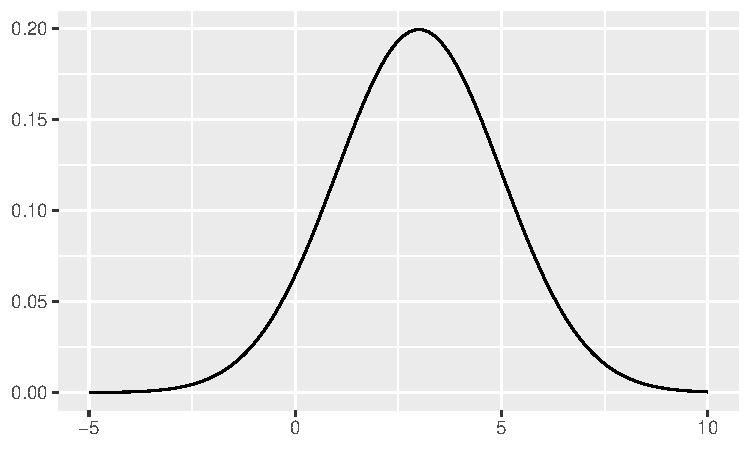
\includegraphics[width=0.6\textwidth]{uncond_dist.pdf}
    \end{center}
    \vspace{-2ex}
    What is the individual-specific coefficient $\beta_n$ for some specific individual?
\end{frame}

\begin{frame}\frametitle{Example of Conditional Distributions}
    \begin{center}
        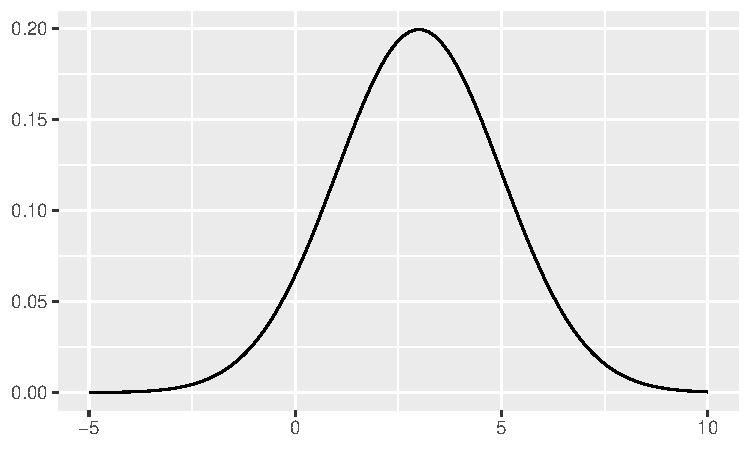
\includegraphics[width=0.6\textwidth]{uncond_dist.pdf}
    \end{center}
    \vspace{-2ex}
    What is the individual-specific coefficient $\beta_n$ for:
    \begin{itemize}
        \item A person drawn randomly from the population?
        \begin{itemize}
            \item The unconditional distribution of $\beta$ in the population, $\beta_n \sim \mathcal{N}(3, 4)$
        \end{itemize}
        \item Someone who regularly drives to work?
        \begin{itemize}
            \item Drivers are more likely to have relatively large values of $\beta_n$
        \end{itemize}
        \item Someone who regularly does not drive to work?
        \begin{itemize}
            \item Non-drivers are more likely to have relative low or negative values of $\beta_n$
        \end{itemize}
    \end{itemize}
\end{frame}

\begin{frame}\frametitle{Example of Conditional Distributions}
    We have described three different distributions for the coefficient $\beta$
    \begin{itemize}
        \item The unconditional distribution for the population (solid line)
        \item The conditional distribution for drivers (dashed line)
        \item The conditional distribution for non-drivers (dotted line)
    \end{itemize}
    \begin{center}
        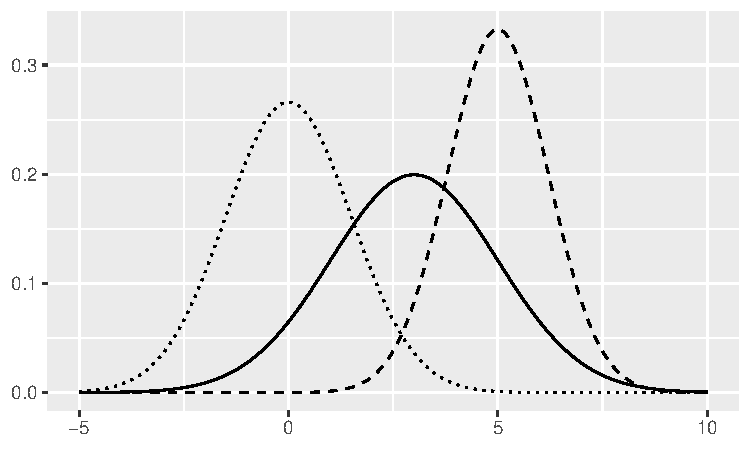
\includegraphics[width=0.8\textwidth]{all_dist.pdf}
    \end{center}
    \vspace{-2ex}
\end{frame}

\begin{frame}\frametitle{Conditional Distribution of Coefficients}
    Suppose that a population of individuals:
    \begin{itemize}
        \item Faces an identical choice setting
        \begin{itemize}
            \item The same choice set, $\{1, 2, \ldots, J\}$, and the same choice attributes, $\bm{x}$
        \end{itemize}
        \item Has heterogeneous preferences denoted by the distribution of coefficients, $f(\bm{\beta} \mid \bm{\theta})$
        \begin{itemize}
            \item This is the unconditional (or population) distribution that we have previously defined
        \end{itemize}
    \end{itemize}
    \vspace{1ex}
    Consider everyone in the population who chooses alternative $i$
    \begin{itemize}
        \item This group is a non-random subset of the population
        \item These individuals also have a distribution of preferences, or $\bm{\beta}_n$ coefficients, but it is likely a different distribution from the population
    \end{itemize}
    \vspace{1ex}
    The distribution of coefficients for this group is called a conditional distribution and is denoted by $h(\bm{\beta} \mid i, \bm{x}, \bm{\theta})$
    \begin{itemize}
        \item Distribution of $\bm{\beta}$ among the group---from a population with an unconditional distribution defined by $\bm{\theta}$---who choose alternative $i$ when faced with choice setting $\bm{x}$
    \end{itemize}
\end{frame}

\section{Derivation of Conditional Distributions}
\label{deriv}
\begin{frame}\frametitle{}
    \vfill
    \centering
    \begin{beamercolorbox}[center]{title}
        \Large Derivation of Conditional Distributions
    \end{beamercolorbox}
    \vfill
\end{frame}

\begin{frame}\frametitle{Random Utility Model with Random Coefficients}
    The utility that decision maker $n$ obtains from alternative $j$ in choice situation $t$ is
    $$U_{njt} = \bm{\beta}_n' \bm{x}_{njt} + \varepsilon_{njt}$$
    \begin{itemize}
    	\item $\bm{x}_{njt}$: data about decision maker $n$ and alternative $j$ in situation $t$
    	\item $\bm{\beta}_n$: individual-specific coefficients with population density $f(\bm{\beta} \mid \bm{\theta})$
    	\item $\varepsilon_{njt}$: i.i.d.\ extreme value random utility term
    \end{itemize}
    \vspace{2ex}
    To simplify notation
    \begin{itemize}
    	\item $\bm{x}_n$: data collectively defined for all alternatives and choice situations
    	\item $\bm{y}_n$: sequence of alternatives chosen by decision maker $n$
    \end{itemize}
\end{frame}

\begin{frame}\frametitle{Choice Probabilities with Random Coefficients}
    If we knew a decision maker's coefficients, $\bm{\beta}_n$, the probability of choosing sequence $\bm{y}_n$ when faced with choice settings $\bm{x}_n$ would be the product of conditional logit choice probabilities
    \begin{align*}
    	P(\bm{y}_n \mid \bm{x}_n, \bm{\beta}_n) & = \prod_{t = 1}^T L_{nt}(y_{nt} \mid \bm{\beta}_n) \\
    	\intertext{where $L_{nt}(y_{nt} \mid \bm{\beta}_n)$ is the conditional logit choice probability}
    	L_{nt}(y_{nt} \mid \bm{\beta}_n) & = \frac{e^{\bm{\beta}_n' \bm{x}_{ny_{nt}t}}}{\sum_{j = 1}^J e^{\bm{\beta}_n' \bm{x}_{njt}}}
    	\intertext{But we do not know each individual's coefficients, $\bm{\beta}_n$, so we have to consider the unconditional distribution of coefficients in the population and intergrate over this density}
    	P(\bm{y}_n \mid \bm{x}_n, \bm{\theta}) & = \int P(\bm{y}_n \mid \bm{x}_n, \bm{\beta}) f(\bm{\beta} \mid \bm{\theta}) d \bm{\beta}
    \end{align*}
\end{frame}

\begin{frame}\frametitle{Joint Density of Choices and Coefficients}
    The integrand of this choice probability is the joint density of $\bm{y}_n$ and $\bm{\beta}$
    $$P(\bm{y}_n \mid \bm{x}_n, \bm{\beta}) \times f(\bm{\beta} \mid \bm{\theta})$$ \\
    \begin{itemize}
        \item Conditional probability of $\bm{y}_n$ times the unconditional density of $\bm{\beta}$
    \end{itemize}
    \vspace{2ex}
    If we reverse the conditioning, we instead get
    $$h(\bm{\beta} \mid \bm{y}_n, \bm{x}_n, \bm{\theta}) \times P(\bm{y}_n \mid \bm{x}_n, \bm{\theta})$$ \\
    \begin{itemize}
        \item Conditional density of $\bm{\beta}$ times the unconditional probability of $\bm{y}_n$
    \end{itemize}
    \vspace{2ex}
    By Bayes' Rule, these two expressions are equal
    $$h(\bm{\beta} \mid \bm{y}_n, \bm{x}_n, \bm{\theta}) \times P(\bm{y}_n \mid \bm{x}_n, \bm{\theta}) = P(\bm{y}_n \mid \bm{x}_n, \bm{\beta}) \times f(\bm{\beta} \mid \bm{\theta})$$
\end{frame}

\begin{frame}\frametitle{Conditional Distribution of Random Coefficients}
    The joint density of $\bm{y}_n$ and $\bm{\beta}$ is either side of the expression
    $$h(\bm{\beta} \mid \bm{y}_n, \bm{x}_n, \bm{\theta}) \times P(\bm{y}_n \mid \bm{x}_n, \bm{\theta}) = P(\bm{y}_n \mid \bm{x}_n, \bm{\beta}) \times f(\bm{\beta} \mid \bm{\theta})$$ \\
    \vspace{2ex}
    Rearranging terms gives an expression for the conditional distribution of $\bm{\beta}$
    $$h(\bm{\beta} \mid \bm{y}_n, \bm{x}_n, \bm{\theta}) = \frac{P(\bm{y}_n \mid \bm{x}_n, \bm{\beta}) \times f(\bm{\beta} \mid \bm{\theta})}{P(\bm{y}_n \mid \bm{x}_n, \bm{\theta})}$$ \\
    \begin{itemize}
        \item The numerator is the integrand of the mixed logit choice probability
        \item The denominator is the mixed logit choice probability
    \end{itemize}
    \vspace{2ex}
    The conditional distribution, $h(\bm{\beta} \mid \bm{y}_n, \bm{x}_n, \bm{\theta})$, is proportional to the product of
    \begin{itemize}
        \item The probability that an individual with coefficients $\bm{\beta}$ would choose $\bm{y}_n$
    	\item The likelihood of observing $\bm{\beta}$ in the population
    \end{itemize}
\end{frame}

\section{Applications of Conditional Distributions}
\label{app}
\begin{frame}\frametitle{}
    \vfill
    \centering
    \begin{beamercolorbox}[center]{title}
        \Large Applications of Conditional Distributions
    \end{beamercolorbox}
    \vfill
\end{frame}

\begin{frame}\frametitle{Conditional Mean Coefficients}
    It is often easier to calculate a statistic derived from the conditional distribution, rather than the conditional distribution itself
    \begin{itemize}
        \item One example is the mean of the conditional distribution, or the conditional mean coefficients
    \end{itemize}
    \vspace{2ex}
    The mean of $h(\bm{\beta} \mid \bm{y}_n, \bm{x}_n, \bm{\theta})$, or the mean of $\bm{\beta}$ among the group---from a population with an unconditional distribution defined by $\bm{\theta}$---who choose sequence $\bm{y}_n$ when faced with choice setting $\bm{x}_n$, is
    \begin{align*}
    	\bar{\bm{\beta}}_n & = \int \bm{\beta} h(\bm{\beta} \mid \bm{y}_n, \bm{x}_n, \bm{\theta}) d \bm{\beta} \\
    	& = \frac{\int \bm{\beta} P(\bm{y}_n \mid \bm{x}_n, \bm{\beta}) f(\bm{\beta} \mid \bm{\theta}) d \bm{\beta}}{\int P(\bm{y}_n \mid \bm{x}_n, \bm{\beta}) f(\bm{\beta} \mid \bm{\theta}) d \bm{\beta}}
    \end{align*} \\
    \vspace{2ex}
    These integrals do not have closed-form expressions and must be simulated
\end{frame}

\begin{frame}\frametitle{Simulating Conditional Mean Coefficients}
    The steps to simulate conditional mean coefficients are similar to the steps we used to simulate mixed logit choice probabilities
    \begin{enumerate}
        \item Draw $R$ random vectors from $f(\bm{\beta} \mid \bm{\theta})$, denoted $\{ \bm{\beta}^1, \bm{\beta}^2, \ldots, \bm{\beta}^R \}$
        \item For each random vector, $\bm{\beta}^r$, calculate the conditional choice probability
        $$P(\bm{y}_n \mid \bm{x}_n, \bm{\beta}^r) = \prod_{t = 1}^T \frac{e^{{\bm{\beta}^r}' \bm{x}_{ny_{nt}t}}}{\sum_{j = 1}^J e^{{\bm{\beta}^r}' \bm{x}_{njt}}}$$
        \item Simulate the conditional mean coefficients as the weighted average of the $R$ random vectors
        \begin{align*}
            \check{\bm{\beta}}_n & = \sum_{r = 1}^R w^r \bm{\beta}^r \\
            \intertext{where the weight of each draw is proportional to $P(\bm{y}_n \mid \bm{x}_n, \bm{\beta}^r)$}
            w^r & = \frac{P(\bm{y}_n \mid \bm{x}_n, \bm{\beta}^r)}{\sum_{r = 1}^R P(\bm{y}_n \mid \bm{x}_n, \bm{\beta}^r)}
        \end{align*}
    \end{enumerate}
\end{frame}

\begin{frame}\frametitle{Individual-Specific Coefficients}
    As the number of observed choices ($T$) increases, the conditional mean coefficients for an individual, $\bar{\bm{\beta}}_n$, converges to the individual-specific coefficients, $\bm{\beta}_n$
    \begin{itemize}
        \item $\bar{\bm{\beta}}_n$ is a consistent estimate of $\bm{\beta}_n$
        $$\bar{\bm{\beta}}_n \overset{p}{\rightarrow} \bm{\beta}_n$$
    \end{itemize}
    \vspace{3ex}
    You must observe (and model) many choices for this convergence to become close
    \begin{itemize}
        \item Train conducts a Monte Carlo simulation exercise to find that even $T = 50$ yields a substantial difference between $\bar{\bm{\beta}}_n$ and $\bm{\beta}_n$
        \item See the Train textbook for more details on this point and the Monte Carlo simulation
    \end{itemize}
\end{frame}

\begin{frame}\frametitle{Future Choice Probabilities}
    If we observe a decision maker's past choices, we can refine future choice probabilities by conditioning on those past choices
    \begin{itemize}
        \item We use the past choices to define a conditional distribution of coefficients for the decision maker
        \item We use this conditional distribution, instead of the unconditional distribution, to calculate mixed logit choice probabilities
    \end{itemize}
    \vspace{2ex}
    The probability that decision maker $n$ chooses alternative $i$ in choice situation $T + 1$ is
    \begin{align*}
    	P(i \mid \bm{x}_{nT+1}, \bm{y}_n, \bm{x}_n, \bm{\theta}) & = \int L_{nT+1} (i \mid \bm{\beta}) h(\bm{\beta} \mid \bm{y}_n, \bm{x}_n, \bm{\theta}) d \bm{\beta}
    	\intertext{where $L_{nT+1} (i \mid \bm{\beta})$ is the conditional logit choice probability}
    	L_{nT+1} (i \mid \bm{\beta}) & = \frac{e^{\bm{\beta}' \bm{x}_{niT+1}}}{\sum_{j = 1}^J e^{\bm{\beta}' \bm{x}_{njT+1}}}
    \end{align*} \\
    \vspace{2ex}
    This is a mixed logit choice probability and must be simulated
\end{frame}

\begin{frame}\frametitle{Simulating Future Choice Probabilities}
    The steps to simulate future choice probabilities are similar to the steps we used to simulate mixed logit choice probabilities
    \begin{enumerate}
        \item Draw $R$ random vectors from $f(\bm{\beta} \mid \bm{\theta})$, denoted $\{ \bm{\beta}^1, \bm{\beta}^2, \ldots, \bm{\beta}^R \}$
        \item For each random vector, $\bm{\beta}^r$, calculate the conditional choice probability for the first $T$ situations, $P(\bm{y}_n \mid \bm{x}_n, \bm{\beta}^r)$, and the conditional logit choice probabilities for situation $T + 1$, $L_{nT+1} (i \mid \bm{\beta}^r)$
        \item Simulate the future mixed logit choice probabilities as the weighted average of $L_{nT+1} (i \mid \bm{\beta}^r)$
        \begin{align*}
            & \check{P}_{niT+1}(\bm{y}_n, \bm{x}_n, \bm{\theta}) = \sum_{r = 1}^R w^r L_{nT+1}(i \mid \bm{\beta}^r)\\
            \intertext{where the weight of each draw is proportional to $P(\bm{y}_n \mid \bm{x}_n, \bm{\beta}^r)$}
            & w^r = \frac{P(\bm{y}_n \mid \bm{x}_n, \bm{\beta}^r)}{\sum_{r = 1}^R P(\bm{y}_n \mid \bm{x}_n, \bm{\beta}^r)}
        \end{align*}
    \end{enumerate}
\end{frame}

\section{Individual-Level Coefficients R Example}
\label{example}
\begin{frame}\frametitle{}
    \vfill
    \centering
    \begin{beamercolorbox}[center]{title}
        \Large Individual-Level Coefficients R Example
    \end{beamercolorbox}
    \vfill
\end{frame}

\begin{frame}\frametitle{Maximum Simulated Likelihood Estimation Example}
    We are again studying how consumers make choices about expensive and highly energy-consuming systems in their homes
    \begin{itemize}
        \item We have (real) data on 250 households in California and the type of HVAC (heating, ventilation, and air conditioning) system in their home. Each household has the following choice set, and we observe the following data
    \end{itemize}
    \vspace{2ex}
    \begin{columns}
        \begin{column}{0.5\textwidth}
            Choice set
            \begin{itemize}
                \item \texttt{ec}: electric central
                \item \texttt{ecc}: electric central with AC
                \item \texttt{er}: electric room
                \item \texttt{erc}: electric room with AC
                \item \texttt{gc}: gas central
                \item \texttt{gcc}: gas central with AC
                \item \texttt{hpc}: heat pump with AC
            \end{itemize}
        \end{column}
        \begin{column}{0.5\textwidth}
            Alternative-specific data
            \begin{itemize}
                \item \texttt{ich}: installation cost for heat
                \item \texttt{icca}: installation cost for AC
                \item \texttt{och}: operating cost for heat
                \item \texttt{occa}: operating cost for AC
            \end{itemize}
            \vspace{2ex}
            Household demographic data
            \begin{itemize}
                \item \texttt{income}: annual income
            \end{itemize}
            \vspace{1ex}
        \end{column}
    \end{columns}
\end{frame}

\begin{frame}[fragile]\frametitle{Load Dataset}
\begin{knitrout}\footnotesize
\definecolor{shadecolor}{rgb}{0.969, 0.969, 0.969}\color{fgcolor}\begin{kframe}
\begin{alltt}
\hlcom{## Load tidyverse and mlogit}
\hlkwd{library}\hlstd{(tidyverse)}
\hlkwd{library}\hlstd{(mlogit)}
\hlcom{## Load dataset from mlogit package}
\hlkwd{data}\hlstd{(}\hlstr{'HC'}\hlstd{,} \hlkwc{package} \hlstd{=} \hlstr{'mlogit'}\hlstd{)}
\end{alltt}
\end{kframe}
\end{knitrout}
\end{frame}

\begin{frame}[fragile]\frametitle{Dataset}
\begin{knitrout}\footnotesize
\definecolor{shadecolor}{rgb}{0.969, 0.969, 0.969}\color{fgcolor}\begin{kframe}
\begin{alltt}
\hlcom{## Look at dataset}
\hlkwd{tibble}\hlstd{(HC)}
\end{alltt}
\begin{verbatim}
## # A tibble: 250 x 18
##    depvar ich.gcc ich.ecc ich.erc ich.hpc ich.gc ich.ec ich.er  icca
##    <fct>    <dbl>   <dbl>   <dbl>   <dbl>  <dbl>  <dbl>  <dbl> <dbl>
##  1 erc       9.7     7.86    8.79   11.4    24.1   24.5   7.37  27.3
##  2 hpc       8.77    8.69    7.09    9.37   28     32.7   9.33  26.5
##  3 gcc       7.43    8.86    6.94   11.7    25.7   31.7   8.14  22.6
##  4 gcc       9.18    8.93    7.22   12.1    29.7   26.7   8.04  25.3
##  5 gcc       8.05    7.02    8.44   10.5    23.9   28.4   7.15  25.4
##  6 gcc       9.32    8.03    6.22   12.6    27.0   21.4   8.6   19.9
##  7 gc        7.11    8.78    7.36   12.4    22.9   28.6   6.41  27.0
##  8 hpc       9.38    7.48    6.72    8.93   26.2   27.9   7.3   18.1
##  9 gcc       8.08    7.39    8.79   11.2    23.0   22.6   7.85  22.6
## 10 gcc       6.24    4.88    7.46    8.28   19.8   27.5   6.88  25.8
## # ... with 240 more rows, and 9 more variables: och.gcc <dbl>,
## #   och.ecc <dbl>, och.erc <dbl>, och.hpc <dbl>, och.gc <dbl>,
## #   och.ec <dbl>, och.er <dbl>, occa <dbl>, income <dbl>
\end{verbatim}
\end{kframe}
\end{knitrout}
\end{frame}

\begin{frame}[fragile]\frametitle{Format Dataset in a Long Format}
\begin{knitrout}\footnotesize
\definecolor{shadecolor}{rgb}{0.969, 0.969, 0.969}\color{fgcolor}\begin{kframe}
\begin{alltt}
\hlcom{## Pivot into a long dataset}
\hlstd{hvac_long} \hlkwb{<-} \hlstd{HC} \hlopt
  \hlkwd{mutate}\hlstd{(}\hlkwc{id} \hlstd{=} \hlnum{1}\hlopt{:}\hlkwd{n}\hlstd{())} \hlopt
  \hlkwd{pivot_longer}\hlstd{(}\hlkwd{c}\hlstd{(}\hlkwd{starts_with}\hlstd{(}\hlstr{'ich.'}\hlstd{),} \hlkwd{starts_with}\hlstd{(}\hlstr{'och.'}\hlstd{)),}
               \hlkwc{names_to} \hlstd{=} \hlkwd{c}\hlstd{(}\hlstr{'cost'}\hlstd{,} \hlstr{'alt'}\hlstd{),} \hlkwc{names_sep} \hlstd{=} \hlstr{'[.]'}\hlstd{,}
               \hlkwc{values_to} \hlstd{=} \hlstr{'value'}\hlstd{)} \hlopt
  \hlkwd{pivot_wider}\hlstd{(}\hlkwc{names_from} \hlstd{= cost,} \hlkwc{values_from} \hlstd{= value)} \hlopt
  \hlkwd{mutate}\hlstd{(}\hlkwc{choice} \hlstd{= (depvar} \hlopt{==} \hlstd{alt))} \hlopt
  \hlkwd{select}\hlstd{(}\hlopt{-}\hlstd{depvar)}
\end{alltt}
\end{kframe}
\end{knitrout}
\end{frame}

\begin{frame}[fragile]\frametitle{Dataset in a Long Format}
\begin{knitrout}\footnotesize
\definecolor{shadecolor}{rgb}{0.969, 0.969, 0.969}\color{fgcolor}\begin{kframe}
\begin{alltt}
\hlcom{## Look at long dataset}
\hlkwd{tibble}\hlstd{(hvac_long)}
\end{alltt}
\begin{verbatim}
## # A tibble: 1,750 x 8
##     icca  occa income    id alt     ich   och choice
##    <dbl> <dbl>  <dbl> <int> <chr> <dbl> <dbl> <lgl> 
##  1  27.3  2.95     20     1 gcc    9.7   2.26 FALSE 
##  2  27.3  2.95     20     1 ecc    7.86  4.09 FALSE 
##  3  27.3  2.95     20     1 erc    8.79  3.85 TRUE  
##  4  27.3  2.95     20     1 hpc   11.4   1.73 FALSE 
##  5  27.3  2.95     20     1 gc    24.1   2.26 FALSE 
##  6  27.3  2.95     20     1 ec    24.5   4.09 FALSE 
##  7  27.3  2.95     20     1 er     7.37  3.85 FALSE 
##  8  26.5  1.63     50     2 gcc    8.77  2.3  FALSE 
##  9  26.5  1.63     50     2 ecc    8.69  2.69 FALSE 
## 10  26.5  1.63     50     2 erc    7.09  3.45 FALSE 
## # ... with 1,740 more rows
\end{verbatim}
\end{kframe}
\end{knitrout}
\end{frame}

\begin{frame}[fragile]\frametitle{Clean Dataset}
\begin{knitrout}\footnotesize
\definecolor{shadecolor}{rgb}{0.969, 0.969, 0.969}\color{fgcolor}\begin{kframe}
\begin{alltt}
\hlcom{## Combine heating and cooling costs into one variable}
\hlstd{hvac_clean} \hlkwb{<-} \hlstd{hvac_long} \hlopt
  \hlkwd{mutate}\hlstd{(}\hlkwc{ac} \hlstd{=} \hlnum{1} \hlopt{*} \hlstd{(}\hlkwd{nchar}\hlstd{(alt)} \hlopt{==} \hlnum{3}\hlstd{),}
         \hlkwc{ic} \hlstd{= ich} \hlopt{+} \hlstd{ac} \hlopt{*} \hlstd{icca,}
         \hlkwc{oc} \hlstd{= och} \hlopt{+} \hlstd{ac} \hlopt{*} \hlstd{occa)} \hlopt
  \hlkwd{select}\hlstd{(id, alt, choice, ac, ic, oc, income)} \hlopt
  \hlkwd{arrange}\hlstd{(id, alt)}
\end{alltt}
\end{kframe}
\end{knitrout}
\end{frame}

\begin{frame}[fragile]\frametitle{Cleaned Dataset}
\begin{knitrout}\footnotesize
\definecolor{shadecolor}{rgb}{0.969, 0.969, 0.969}\color{fgcolor}\begin{kframe}
\begin{alltt}
\hlcom{## Look at cleaned dataset}
\hlkwd{tibble}\hlstd{(hvac_clean)}
\end{alltt}
\begin{verbatim}
## # A tibble: 1,750 x 7
##       id alt   choice    ac    ic    oc income
##    <int> <chr> <lgl>  <dbl> <dbl> <dbl>  <dbl>
##  1     1 ec    FALSE      0 24.5   4.09     20
##  2     1 ecc   FALSE      1 35.1   7.04     20
##  3     1 er    FALSE      0  7.37  3.85     20
##  4     1 erc   TRUE       1 36.1   6.8      20
##  5     1 gc    FALSE      0 24.1   2.26     20
##  6     1 gcc   FALSE      1 37.0   5.21     20
##  7     1 hpc   FALSE      1 38.6   4.68     20
##  8     2 ec    FALSE      0 32.7   2.69     50
##  9     2 ecc   FALSE      1 35.2   4.32     50
## 10     2 er    FALSE      0  9.33  3.45     50
## # ... with 1,740 more rows
\end{verbatim}
\end{kframe}
\end{knitrout}
\end{frame}

\begin{frame}[fragile]\frametitle{Convert Dataset to \texttt{dfidx} Format}
\begin{knitrout}\footnotesize
\definecolor{shadecolor}{rgb}{0.969, 0.969, 0.969}\color{fgcolor}\begin{kframe}
\begin{alltt}
\hlcom{## Convert cleaned dataset to dfidx format}
\hlstd{hvac_dfidx} \hlkwb{<-} \hlkwd{dfidx}\hlstd{(hvac_clean,} \hlkwc{shape} \hlstd{=} \hlstr{'long'}\hlstd{,}
                    \hlkwc{choice} \hlstd{=} \hlstr{'choice'}\hlstd{,} \hlkwc{idx} \hlstd{=} \hlkwd{c}\hlstd{(}\hlstr{'id'}\hlstd{,} \hlstr{'alt'}\hlstd{))}
\end{alltt}
\end{kframe}
\end{knitrout}
\end{frame}

\begin{frame}[fragile]\frametitle{Dataset in \texttt{dfidx} Format}
\begin{knitrout}\footnotesize
\definecolor{shadecolor}{rgb}{0.969, 0.969, 0.969}\color{fgcolor}\begin{kframe}
\begin{alltt}
\hlcom{## Look at data in dfidx format}
\hlkwd{tibble}\hlstd{(hvac_dfidx)}
\end{alltt}
\begin{verbatim}
## # A tibble: 1,750 x 6
##    choice    ac    ic    oc income idx$id $alt 
##    <lgl>  <dbl> <dbl> <dbl>  <dbl>  <int> <fct>
##  1 FALSE      0 24.5   4.09     20      1 ec   
##  2 FALSE      1 35.1   7.04     20      1 ecc  
##  3 FALSE      0  7.37  3.85     20      1 er   
##  4 TRUE       1 36.1   6.8      20      1 erc  
##  5 FALSE      0 24.1   2.26     20      1 gc   
##  6 FALSE      1 37.0   5.21     20      1 gcc  
##  7 FALSE      1 38.6   4.68     20      1 hpc  
##  8 FALSE      0 32.7   2.69     50      2 ec   
##  9 FALSE      1 35.2   4.32     50      2 ecc  
## 10 FALSE      0  9.33  3.45     50      2 er   
## # ... with 1,740 more rows
\end{verbatim}
\end{kframe}
\end{knitrout}
\end{frame}

\begin{frame}\frametitle{Mixed Logit Model of HVAC System Choice}
    We previously estimated a mixed logit model with representative utility
    $$V_{nj} = \beta_{1n} AC_j + \beta_{2n} IC_{nj} + \beta_{3n} OC_{nj}$$
    where the random coefficients are normally distributed
    \begin{align*}
        \beta_{1n} & \sim \mathcal{N}(\mu_1, \sigma_1^2) \\
        \beta_{2n} & \sim \mathcal{N}(\mu_2, \sigma_2^2) \\
        \beta_{3n} & \sim \mathcal{N}(\mu_3, \sigma_3^2)
    \end{align*}
\end{frame}

\begin{frame}\frametitle{Conditional Mean Coefficients for HVAC System Choice}
    The public utility commission is considering a subsidy on the installation cost of heat pump systems to incentivize households to switch to this most efficient HVAC system
    \begin{itemize}
        \item The PUC would like to target this subsidy and its marketing to households with certain HVAC system preferences
        \item We can use information about the HVAC system that a household currently has to generate a conditional distribution of coefficients that better describes that household's preferences
    \end{itemize}
    \vspace{2ex}
    For each alternative, what are the mean $\bm{\beta}_n$ coefficients for the households with that HVAC system?
    \begin{enumerate}
        \item Estimate the mixed logit model
        \item Simulate $\check{\bm{\beta}}_n$ for each household
        \item Average $\check{\bm{\beta}}_n$ for the households with each HVAC system
    \end{enumerate}
\end{frame}

\begin{frame}\frametitle{Simulating Conditional Mean Coefficients}
    Two ways to simulate conditional mean coefficients for each household
    \begin{itemize}
        \item \texttt{mlogit} package
        \item Code the simulation by hand
    \end{itemize}
    \vspace{3ex}
    The \texttt{fitted()} function with \texttt{type = `parameters'} simulates the conditional mean coefficients for every individual
    \begin{itemize}
        \item This function returns the $N \times K$ matrix of conditional mean coefficients
    \end{itemize}
    \vspace{3ex}
    We can instead code the simulation by hand
    \begin{itemize}
        \item We may want to simulate additional objects that are not part of the \texttt{mlogit} functionality
    \end{itemize}
\end{frame}

\begin{frame}[fragile]\frametitle{Mixed Logit Model Using \texttt{mlogit}}
\begin{knitrout}\footnotesize
\definecolor{shadecolor}{rgb}{0.969, 0.969, 0.969}\color{fgcolor}\begin{kframe}
\begin{alltt}
\hlcom{## Model choice using ac, ic, and oc with normal random coefficients}
\hlstd{model_1} \hlkwb{<-} \hlkwd{mlogit}\hlstd{(}\hlkwc{formula} \hlstd{= choice} \hlopt{~} \hlstd{ac} \hlopt{+} \hlstd{ic} \hlopt{+} \hlstd{oc} \hlopt{|} \hlnum{0} \hlopt{|} \hlnum{0}\hlstd{,}
                  \hlkwc{data} \hlstd{= hvac_dfidx,}
                  \hlkwc{reflevel} \hlstd{=} \hlstr{'hpc'}\hlstd{,}
                  \hlkwc{rpar} \hlstd{=} \hlkwd{c}\hlstd{(}\hlkwc{ac} \hlstd{=} \hlstr{'n'}\hlstd{,} \hlkwc{ic} \hlstd{=} \hlstr{'n'}\hlstd{,} \hlkwc{oc} \hlstd{=} \hlstr{'n'}\hlstd{),}
                  \hlkwc{R} \hlstd{=} \hlnum{1000}\hlstd{,} \hlkwc{seed} \hlstd{=} \hlnum{703}\hlstd{)}
\end{alltt}
\end{kframe}
\end{knitrout}
\end{frame}

\begin{frame}[fragile]\frametitle{Mixed Logit Model Results Using \texttt{mlogit}}
    \vspace{1ex}
\begin{knitrout}\tiny
\definecolor{shadecolor}{rgb}{0.969, 0.969, 0.969}\color{fgcolor}\begin{kframe}
\begin{alltt}
\hlcom{## Summarize model results}
\hlkwd{summary}\hlstd{(model_1)}
\end{alltt}
\begin{verbatim}
## 
## Call:
## mlogit(formula = choice ~ ac + ic + oc | 0 | 0, data = hvac_dfidx, 
##     reflevel = "hpc", rpar = c(ac = "n", ic = "n", oc = "n"), 
##     R = 1000, seed = 703)
## 
## Frequencies of alternatives:choice
##   hpc    ec   ecc    er   erc    gc   gcc 
## 0.104 0.004 0.016 0.032 0.004 0.096 0.744 
## 
## bfgs method
## 22 iterations, 0h:0m:53s 
## g'(-H)^-1g = 7.26E-07 
## gradient close to zero 
## 
## Coefficients :
##         Estimate Std. Error z-value  Pr(>|z|)    
## ac    10.8829832  3.8264644  2.8441  0.004453 ** 
## ic    -0.2150971  0.0349316 -6.1577 7.382e-10 ***
## oc    -1.1233808  0.1865858 -6.0207 1.736e-09 ***
## sd.ac  4.4597527  3.6209211  1.2317  0.218075    
## sd.ic  0.0010176  0.3371230  0.0030  0.997592    
## sd.oc  0.0110849  1.7285017  0.0064  0.994883    
## ---
## Signif. codes:  0 '***' 0.001 '**' 0.01 '*' 0.05 '.' 0.1 ' ' 1
## 
## Log-Likelihood: -327.22
## 
## random coefficients
##    Min.    1st Qu.     Median       Mean    3rd Qu. Max.
## ac -Inf  7.8749258 10.8829832 10.8829832 13.8910407  Inf
## ic -Inf -0.2157834 -0.2150971 -0.2150971 -0.2144107  Inf
## oc -Inf -1.1308575 -1.1233808 -1.1233808 -1.1159042  Inf
\end{verbatim}
\end{kframe}
\end{knitrout}
\end{frame}

\begin{frame}[fragile]\frametitle{Conditional Mean Coefficients Using \texttt{mlogit}}
\begin{knitrout}\footnotesize
\definecolor{shadecolor}{rgb}{0.969, 0.969, 0.969}\color{fgcolor}\begin{kframe}
\begin{alltt}
\hlcom{## Calculate mean coefficient for each household}
\hlstd{coefs_1} \hlkwb{<-} \hlstd{model_1} \hlopt
  \hlkwd{fitted}\hlstd{(}\hlkwc{type} \hlstd{=} \hlstr{'parameters'}\hlstd{)} \hlopt
  \hlkwd{as_tibble}\hlstd{()} \hlopt
  \hlkwd{rename}\hlstd{(}\hlkwc{ac_coef} \hlstd{= ac,} \hlkwc{ic_coef} \hlstd{= ic,} \hlkwc{oc_coef} \hlstd{= oc)}
\hlstd{coefs_1}
\end{alltt}
\begin{verbatim}
## # A tibble: 250 x 3
##    ac_coef ic_coef oc_coef
##      <dbl>   <dbl>   <dbl>
##  1   12.4   -0.215   -1.12
##  2   11.8   -0.215   -1.12
##  3   11.8   -0.215   -1.12
##  4   12.0   -0.215   -1.12
##  5   12.5   -0.215   -1.12
##  6   11.6   -0.215   -1.12
##  7    4.44  -0.215   -1.12
##  8   11.6   -0.215   -1.12
##  9   11.8   -0.215   -1.12
## 10   11.7   -0.215   -1.12
## # ... with 240 more rows
\end{verbatim}
\end{kframe}
\end{knitrout}
\end{frame}

\begin{frame}[fragile]\frametitle{Average Conditional Mean Coefficients Using \texttt{mlogit}}
\begin{knitrout}\footnotesize
\definecolor{shadecolor}{rgb}{0.969, 0.969, 0.969}\color{fgcolor}\begin{kframe}
\begin{alltt}
\hlcom{## Average coefficient over all households with each HVAC system}
\hlstd{hvac_clean} \hlopt
  \hlkwd{filter}\hlstd{(choice} \hlopt{==} \hlnum{1}\hlstd{)} \hlopt
  \hlkwd{cbind}\hlstd{(coefs_1)} \hlopt
  \hlkwd{group_by}\hlstd{(alt)} \hlopt
  \hlkwd{summarize}\hlstd{(}\hlkwc{ac_coef} \hlstd{=} \hlkwd{mean}\hlstd{(ac_coef),}
            \hlkwc{ic_coef} \hlstd{=} \hlkwd{mean}\hlstd{(ic_coef),}
            \hlkwc{oc_coef} \hlstd{=} \hlkwd{mean}\hlstd{(oc_coef),}
            \hlkwc{.groups} \hlstd{=} \hlstr{'drop'}\hlstd{)}
\end{alltt}
\begin{verbatim}
## # A tibble: 7 x 4
##   alt   ac_coef ic_coef oc_coef
##   <chr>   <dbl>   <dbl>   <dbl>
## 1 ec       4.40  -0.215   -1.12
## 2 ecc     11.9   -0.215   -1.12
## 3 er       4.35  -0.215   -1.12
## 4 erc     12.4   -0.215   -1.12
## 5 gc       4.30  -0.215   -1.12
## 6 gcc     11.9   -0.215   -1.12
## 7 hpc     11.9   -0.215   -1.12
\end{verbatim}
\end{kframe}
\end{knitrout}
\end{frame}

\begin{frame}\frametitle{Steps for Simulating Conditional Mean Coefficients}
    $$\check{\bm{\beta}}_n = \frac{\sum_{r = 1}^R \bm{\beta}^r P(y_n \mid \bm{x}_n, \bm{\beta}^r)}{\sum_{r = 1}^R P(y_n \mid \bm{x}_n, \bm{\beta}^r)}$$
    \begin{enumerate}
        \item Draw $K \times N \times R$ standard normal random variables
        \begin{itemize}
            \item $K$ random coefficients for each of
            \item $N$ different decision makers for each of
            \item $R$ different simulation draws
        \end{itemize}
        \item Find the MSL estimator, $\widehat{\bm{\theta}}$
        \begin{itemize}
            \item See slides from last week on MSL estimation
        \end{itemize}
        \item Simulate conditional mean coefficients using the MSL estimator, $\widehat{\bm{\theta}}$
        \begin{enumerate}
            \item Transform each set of $K$ standard normals using $\widehat{\bm{\theta}}$ to get $\bm{\beta}^r$
            \item Calculate the conditional logit choice probability of the chosen alternative, $P(y_n \mid \bm{x}_n, \bm{\beta}^r)$, for each household and random draw
            \item For each household, take a weighted average of $\bm{\beta}^r$, with weights proportional to $P(y_n \mid \bm{x}_n, \bm{\beta}^r)$, to get $\check{\bm{\beta}}_n$
        \end{enumerate}
    \end{enumerate}
\end{frame}

\begin{frame}[fragile]\frametitle{Step 1: Draw Random Variables and Organize Data}
\begin{knitrout}\footnotesize
\definecolor{shadecolor}{rgb}{0.969, 0.969, 0.969}\color{fgcolor}\begin{kframe}
\begin{alltt}
\hlcom{## Set seed for replication}
\hlkwd{set.seed}\hlstd{(}\hlnum{703}\hlstd{)}
\hlcom{## Draw standard normal random variables for each household}
\hlstd{draws_hh} \hlkwb{<-} \hlkwd{map}\hlstd{(}\hlnum{1}\hlopt{:}\hlnum{250}\hlstd{,} \hlopt{~} \hlkwd{tibble}\hlstd{(}\hlkwc{ac_draw} \hlstd{=} \hlkwd{rnorm}\hlstd{(}\hlnum{100}\hlstd{),}
                                \hlkwc{ic_draw} \hlstd{=} \hlkwd{rnorm}\hlstd{(}\hlnum{100}\hlstd{),}
                                \hlkwc{oc_draw} \hlstd{=} \hlkwd{rnorm}\hlstd{(}\hlnum{100}\hlstd{)))}
\hlcom{## Split data into list by household}
\hlstd{data_hh} \hlkwb{<-} \hlstd{hvac_clean} \hlopt
  \hlkwd{group_by}\hlstd{(id)} \hlopt
  \hlkwd{group_split}\hlstd{()}
\end{alltt}
\end{kframe}
\end{knitrout}
\end{frame}

\begin{frame}[fragile]\frametitle{Step 2a: Simulate Choice Probabilities for One Household}
\begin{knitrout}\tiny
\definecolor{shadecolor}{rgb}{0.969, 0.969, 0.969}\color{fgcolor}\begin{kframe}
\begin{alltt}
\hlcom{## Function to simulate choice probabilities for an individual household}
\hlstd{sim_probs_ind} \hlkwb{<-} \hlkwa{function}\hlstd{(}\hlkwc{params}\hlstd{,} \hlkwc{draws_ind}\hlstd{,} \hlkwc{data_ind}\hlstd{)\{}
  \hlcom{## Select relevant variables and convert into a matrix [J x K]}
  \hlstd{data_matrix} \hlkwb{<-} \hlstd{data_ind} \hlopt
    \hlkwd{select}\hlstd{(ac, ic, oc)} \hlopt
    \hlkwd{as.matrix}\hlstd{()}
  \hlcom{## Transform random coefficients based on parameters [R x K]}
  \hlstd{coef_matrix} \hlkwb{<-} \hlstd{draws_ind} \hlopt
    \hlkwd{mutate}\hlstd{(}\hlkwc{ac_coef} \hlstd{= params[}\hlnum{1}\hlstd{]} \hlopt{+} \hlstd{params[}\hlnum{4}\hlstd{]} \hlopt{*} \hlstd{ac_draw,}
           \hlkwc{ic_coef} \hlstd{= params[}\hlnum{2}\hlstd{]} \hlopt{+} \hlstd{params[}\hlnum{5}\hlstd{]} \hlopt{*} \hlstd{ic_draw,}
           \hlkwc{oc_coef} \hlstd{= params[}\hlnum{3}\hlstd{]} \hlopt{+} \hlstd{params[}\hlnum{6}\hlstd{]} \hlopt{*} \hlstd{oc_draw)} \hlopt
    \hlkwd{select}\hlstd{(ac_coef, ic_coef, oc_coef)} \hlopt
    \hlkwd{as.matrix}\hlstd{()}
  \hlcom{## Calculate representative utility for each alternative in each draw [R x J]}
  \hlstd{utility} \hlkwb{<-} \hlstd{(coef_matrix} \hlopt \hlkwd{t}\hlstd{(data_matrix))} \hlopt
    \hlkwd{pmin}\hlstd{(}\hlnum{700}\hlstd{)} \hlopt
    \hlkwd{pmax}\hlstd{(}\hlopt{-}\hlnum{700}\hlstd{)}
  \hlcom{## Sum the exponential of utility over alternatives [R x 1]}
  \hlstd{prob_denom} \hlkwb{<-} \hlstd{utility} \hlopt
    \hlkwd{exp}\hlstd{()} \hlopt
    \hlkwd{rowSums}\hlstd{()}
  \hlcom{## Calculate the conditional probability for each alternative and draw [R x J]}
  \hlstd{cond_prob} \hlkwb{<-} \hlkwd{exp}\hlstd{(utility)} \hlopt{/} \hlstd{prob_denom}
  \hlcom{## Calculate simulated choice probabilities as means over all draws [1 x J]}
  \hlstd{sim_prob} \hlkwb{<-} \hlkwd{colMeans}\hlstd{(cond_prob)}
  \hlcom{## Add simulated probability to initial dataset}
  \hlstd{data_ind_out} \hlkwb{<-} \hlstd{data_ind} \hlopt
    \hlkwd{mutate}\hlstd{(}\hlkwc{prob} \hlstd{= sim_prob)}
  \hlcom{## Return initial dataset with simulated probability variable}
  \hlkwd{return}\hlstd{(data_ind_out)}
\hlstd{\}}
\end{alltt}
\end{kframe}
\end{knitrout}
\end{frame}

\begin{frame}[fragile]\frametitle{Step 2b: Calculate Simulated Log-Likelihood}
\begin{knitrout}\footnotesize
\definecolor{shadecolor}{rgb}{0.969, 0.969, 0.969}\color{fgcolor}\begin{kframe}
\begin{alltt}
\hlcom{## Function to calculate simulated log-likelihood}
\hlstd{sim_ll_fn} \hlkwb{<-} \hlkwa{function}\hlstd{(}\hlkwc{params}\hlstd{,} \hlkwc{draws_list}\hlstd{,} \hlkwc{data_list}\hlstd{)\{}
  \hlcom{## Simulate probabilities for each individual household}
  \hlstd{data_sim_ind} \hlkwb{<-} \hlkwd{map2}\hlstd{(}\hlkwc{.x} \hlstd{= draws_list,} \hlkwc{.y} \hlstd{= data_list,}
                       \hlkwc{.f} \hlstd{=} \hlopt{~} \hlkwd{sim_probs_ind}\hlstd{(}\hlkwc{params} \hlstd{= params,}
                                            \hlkwc{draws_ind} \hlstd{= .x,}
                                            \hlkwc{data_ind} \hlstd{= .y))}
  \hlcom{## Combine individual datasets into one}
  \hlstd{data_sim} \hlkwb{<-} \hlstd{data_sim_ind} \hlopt
    \hlkwd{bind_rows}\hlstd{()}
  \hlcom{## Calculate log of simulated probability for the chosen alternative}
  \hlstd{data_sim} \hlkwb{<-} \hlstd{data_sim} \hlopt
    \hlkwd{filter}\hlstd{(choice} \hlopt{==} \hlnum{TRUE}\hlstd{)} \hlopt
    \hlkwd{mutate}\hlstd{(}\hlkwc{log_prob} \hlstd{=} \hlkwd{log}\hlstd{(prob))}
  \hlcom{## Calculate the simulated log-likelihood}
  \hlstd{sim_ll} \hlkwb{<-} \hlkwd{sum}\hlstd{(data_sim}\hlopt{$}\hlstd{log_prob)}
  \hlcom{## Return the negative of simulated log-likelihood}
  \hlkwd{return}\hlstd{(}\hlopt{-}\hlstd{sim_ll)}
\hlstd{\}}
\end{alltt}
\end{kframe}
\end{knitrout}
\end{frame}

\begin{frame}[fragile]\frametitle{Step 2c: Maximize Simulated Log-Likelihood}
\begin{knitrout}\footnotesize
\definecolor{shadecolor}{rgb}{0.969, 0.969, 0.969}\color{fgcolor}\begin{kframe}
\begin{alltt}
\hlcom{## Maximize the log-likelihood function}
\hlstd{model_2} \hlkwb{<-} \hlkwd{optim}\hlstd{(}\hlkwc{par} \hlstd{=} \hlkwd{c}\hlstd{(}\hlnum{6.53}\hlstd{,} \hlopt{-}\hlnum{0.17}\hlstd{,} \hlopt{-}\hlnum{1.04}\hlstd{,} \hlnum{0}\hlstd{,} \hlnum{0}\hlstd{,} \hlnum{0}\hlstd{),} \hlkwc{fn} \hlstd{= sim_ll_fn,}
                 \hlkwc{draws_list} \hlstd{= draws_hh,} \hlkwc{data_list} \hlstd{= data_hh,}
                 \hlkwc{method} \hlstd{=} \hlstr{'BFGS'}\hlstd{,} \hlkwc{hessian} \hlstd{=} \hlnum{TRUE}\hlstd{,}
                 \hlkwc{control} \hlstd{=} \hlkwd{list}\hlstd{(}\hlkwc{trace} \hlstd{=} \hlnum{1}\hlstd{,} \hlkwc{REPORT} \hlstd{=} \hlnum{5}\hlstd{))}
\end{alltt}
\begin{verbatim}
## initial  value 330.051626 
## iter   5 value 329.842440
## iter  10 value 329.559384
## iter  15 value 326.652634
## iter  20 value 325.961965
## iter  25 value 325.960937
## final  value 325.959722 
## converged
\end{verbatim}
\end{kframe}
\end{knitrout}
\end{frame}

\begin{frame}[fragile]\frametitle{Step 2d: Report MSLE Results}
    
\begin{knitrout}\tiny
\definecolor{shadecolor}{rgb}{0.969, 0.969, 0.969}\color{fgcolor}\begin{kframe}
\begin{alltt}
\hlcom{## Report model results}
\hlstd{model_2}
\end{alltt}
\begin{verbatim}
## $par
## [1] 11.0917037025 -0.2164020694 -1.1278947803  4.5934515313  0.0002048493  0.0057092340
## 
## $value
## [1] 325.9597
## 
## $counts
## function gradient 
##       94       28 
## 
## $convergence
## [1] 0
## 
## $message
## NULL
## 
## $hessian
##            [,1]        [,2]        [,3]        [,4]        [,5]        [,6]
## [1,]  4.0451882   95.551233    3.536574  -4.1442779    3.285546   0.2552387
## [2,] 95.5512329 4130.546546 -215.794416 -92.6246226  122.374461   9.2682826
## [3,]  3.5365739 -215.794416  144.136869  -3.9213534   -5.159820   1.3656793
## [4,] -4.1442779  -92.624623   -3.921353   4.4151970   -7.345430  -0.2337583
## [5,]  3.2855456  122.374461   -5.159820  -7.3454298 2686.692261 -15.9361930
## [6,]  0.2552387    9.268283    1.365679  -0.2337583  -15.936193  42.8194368
\end{verbatim}
\end{kframe}
\end{knitrout}
\end{frame}

\begin{frame}[fragile]\frametitle{Step 3a: Simulate Coefficients for One Household}
    $$\check{\bm{\beta}}_n = \frac{\sum_{r = 1}^R \bm{\beta}^r P(y_n \mid \bm{x}_n, \bm{\beta}^r)}{\sum_{r = 1}^R P(y_n \mid \bm{x}_n, \bm{\beta}^r)}$$
\begin{knitrout}\tiny
\definecolor{shadecolor}{rgb}{0.969, 0.969, 0.969}\color{fgcolor}\begin{kframe}
\begin{alltt}
\hlcom{## Function to simulate individual coefficients for one individual}
\hlstd{calc_mean_coefs} \hlkwb{<-} \hlkwa{function}\hlstd{(}\hlkwc{params}\hlstd{,} \hlkwc{draws_ind}\hlstd{,} \hlkwc{data_ind}\hlstd{)\{}
  \hlcom{## Select relevant variables and convert into a matrix [J x K]}
  \hlstd{data_matrix} \hlkwb{<-} \hlstd{data_ind} \hlopt
    \hlkwd{select}\hlstd{(ac, ic, oc)} \hlopt
    \hlkwd{as.matrix}\hlstd{()}
  \hlcom{## Transform random draws into coefficients based on parameters}
  \hlstd{coef} \hlkwb{<-} \hlstd{draws_ind} \hlopt
    \hlkwd{mutate}\hlstd{(}\hlkwc{ac_coef} \hlstd{= params[}\hlnum{1}\hlstd{]} \hlopt{+} \hlstd{params[}\hlnum{4}\hlstd{]} \hlopt{*} \hlstd{ac_draw,}
           \hlkwc{ic_coef} \hlstd{= params[}\hlnum{2}\hlstd{]} \hlopt{+} \hlstd{params[}\hlnum{5}\hlstd{]} \hlopt{*} \hlstd{ic_draw,}
           \hlkwc{oc_coef} \hlstd{= params[}\hlnum{3}\hlstd{]} \hlopt{+} \hlstd{params[}\hlnum{6}\hlstd{]} \hlopt{*} \hlstd{oc_draw)} \hlopt
    \hlkwd{select}\hlstd{(ac_coef, ic_coef, oc_coef)}
  \hlcom{## Convert coefficients tibble to a matrix [R x K]}
  \hlstd{coef_matrix} \hlkwb{<-} \hlkwd{as.matrix}\hlstd{(coef)}
  \hlcom{## Calculate representative utility for each alternative in each draw [R x J]}
  \hlstd{utility} \hlkwb{<-} \hlstd{(coef_matrix} \hlopt \hlkwd{t}\hlstd{(data_matrix))} \hlopt
    \hlkwd{pmin}\hlstd{(}\hlnum{700}\hlstd{)} \hlopt
    \hlkwd{pmax}\hlstd{(}\hlopt{-}\hlnum{700}\hlstd{)}
  \hlcom{## Sum the exponential of utility over alternatives [R x 1]}
  \hlstd{prob_denom} \hlkwb{<-} \hlstd{utility} \hlopt
    \hlkwd{exp}\hlstd{()} \hlopt
    \hlkwd{rowSums}\hlstd{()}
  \hlcom{## Calculate the conditional probability for each alternative and draw [R x J]}
  \hlstd{cond_prob} \hlkwb{<-} \hlkwd{exp}\hlstd{(utility)} \hlopt{/} \hlstd{prob_denom}
  \hlcom{## Calculate the numerator of the draw weights as prob of chosen alt [R x 1]}
  \hlstd{weights_num} \hlkwb{<-} \hlkwd{c}\hlstd{(cond_prob} \hlopt \hlstd{data_ind}\hlopt{$}\hlstd{choice)}
  \hlcom{## Calculate the draw weights [R x 1]}
  \hlstd{weights} \hlkwb{<-} \hlstd{weights_num} \hlopt{/} \hlkwd{sum}\hlstd{(weights_num)}
  \hlcom{## Add draw weights to dataset of coefficients}
  \hlstd{coef} \hlkwb{<-} \hlstd{coef} \hlopt
    \hlkwd{mutate}\hlstd{(}\hlkwc{weight} \hlstd{= weights)}
  \hlcom{## Calculate weighted mean for each coefficient}
  \hlstd{coef_means} \hlkwb{<-} \hlstd{coef} \hlopt
    \hlkwd{summarize}\hlstd{(}\hlkwc{ac_coef_mean} \hlstd{=} \hlkwd{sum}\hlstd{(ac_coef} \hlopt{*} \hlstd{weight),}
              \hlkwc{ic_coef_mean} \hlstd{=} \hlkwd{sum}\hlstd{(ic_coef} \hlopt{*} \hlstd{weight),}
              \hlkwc{oc_coef_mean} \hlstd{=} \hlkwd{sum}\hlstd{(oc_coef} \hlopt{*} \hlstd{weight))}
  \hlcom{## Add individual coefficient means to initial dataset}
  \hlstd{data_ind_out} \hlkwb{<-} \hlstd{data_ind} \hlopt
    \hlkwd{bind_cols}\hlstd{(coef_means)}
  \hlcom{## Return initial dataset with simulated probability variable}
  \hlkwd{return}\hlstd{(data_ind_out)}
\hlstd{\}}
\end{alltt}
\end{kframe}
\end{knitrout}
\end{frame}

\begin{frame}[fragile]\frametitle{Step 3a: Simulate Coefficients for One Household}
    $$\check{\bm{\beta}}_n = \frac{\sum_{r = 1}^R \bm{\beta}^r P(y_n \mid \bm{x}_n, \bm{\beta}^r)}{\sum_{r = 1}^R P(y_n \mid \bm{x}_n, \bm{\beta}^r)}$$
\begin{knitrout}\tiny
\definecolor{shadecolor}{rgb}{0.969, 0.969, 0.969}\color{fgcolor}\begin{kframe}
\begin{alltt}
\hlcom{  ## Sum the exponential of utility over alternatives [R x 1]}
  prob_denom <- utility %>% 
    \hlkwd{exp}() %>% 
    \hlkwd{rowSums}()
\hlcom{  ## Calculate the conditional probability for each alternative and draw [R x J]}
  cond_prob <- \hlkwd{exp}(utility) / prob_denom
\hlcom{  ## Calculate the numerator of the draw weights as prob of chosen alt [R x 1]}
  weights_num <- \hlkwd{c}(cond_prob %*% data_ind$choice)
\hlcom{  ## Calculate the draw weights [R x 1]}
  weights <- weights_num / \hlkwd{sum}(weights_num)
\hlcom{  ## Add draw weights to dataset of coefficients}
  coef <- coef %>%
    \hlkwd{mutate}(weight = weights)
\hlcom{  ## Calculate weighted mean for each coefficient}
  coef_means <- coef %>%
    \hlkwd{summarize}(ac_coef_mean = \hlkwd{sum}(ac_coef * weight),
              ic_coef_mean = \hlkwd{sum}(ic_coef * weight),
              oc_coef_mean = \hlkwd{sum}(oc_coef * weight))
\hlcom{  ## Add individual coefficient means to initial dataset}
  data_ind_out <- data_ind %>% 
    \hlkwd{bind_cols}(coef_means)
\hlcom{  ## Return initial dataset with simulated probability variable}
  \hlkwd{return}(data_ind_out)
\}
\end{alltt}
\end{kframe}
\end{knitrout}
\end{frame}

\begin{frame}[fragile]\frametitle{Step 3b: Simulate Coefficients for All Households}
    $$\check{\bm{\beta}}_n = \frac{\sum_{r = 1}^R \bm{\beta}^r P(y_n \mid \bm{x}_n, \bm{\beta}^r)}{\sum_{r = 1}^R P(y_n \mid \bm{x}_n, \bm{\beta}^r)}$$
\begin{knitrout}\footnotesize
\definecolor{shadecolor}{rgb}{0.969, 0.969, 0.969}\color{fgcolor}\begin{kframe}
\begin{alltt}
\hlcom{## Calculate mean coefficients for each individual}
\hlstd{data_2_ind} \hlkwb{<-} \hlkwd{map2}\hlstd{(}\hlkwc{.x} \hlstd{= draws_hh,} \hlkwc{.y} \hlstd{= data_hh,}
                   \hlkwc{.f} \hlstd{=} \hlopt{~} \hlkwd{calc_mean_coefs}\hlstd{(}\hlkwc{params} \hlstd{= model_2}\hlopt{$}\hlstd{par,}
                                          \hlkwc{draws_ind} \hlstd{= .x,}
                                          \hlkwc{data_ind} \hlstd{= .y))}
\hlcom{## Combine list of data into one tibble}
\hlstd{data_2} \hlkwb{<-} \hlstd{data_2_ind} \hlopt
  \hlkwd{bind_rows}\hlstd{()}
\end{alltt}
\end{kframe}
\end{knitrout}
\end{frame}

\begin{frame}[fragile]\frametitle{Conditional Mean Coefficients for Each HVAC System}
\begin{knitrout}\footnotesize
\definecolor{shadecolor}{rgb}{0.969, 0.969, 0.969}\color{fgcolor}\begin{kframe}
\begin{alltt}
\hlcom{## Calculate mean coefficients by chosen alternative}
\hlstd{data_2} \hlopt
  \hlkwd{filter}\hlstd{(choice} \hlopt{==} \hlnum{1}\hlstd{)} \hlopt
  \hlkwd{group_by}\hlstd{(alt)} \hlopt
  \hlkwd{summarize}\hlstd{(}\hlkwc{ac_coef} \hlstd{=} \hlkwd{mean}\hlstd{(ac_coef_mean),}
            \hlkwc{ic_coef} \hlstd{=} \hlkwd{mean}\hlstd{(ic_coef_mean),}
            \hlkwc{oc_coef} \hlstd{=} \hlkwd{mean}\hlstd{(oc_coef_mean),}
            \hlkwc{.groups} \hlstd{=} \hlstr{'drop'}\hlstd{)}
\end{alltt}
\begin{verbatim}
## # A tibble: 7 x 4
##   alt   ac_coef ic_coef oc_coef
##   <chr>   <dbl>   <dbl>   <dbl>
## 1 ec       4.05  -0.216   -1.13
## 2 ecc     12.3   -0.216   -1.13
## 3 er       4.39  -0.216   -1.13
## 4 erc     12.1   -0.216   -1.13
## 5 gc       4.20  -0.216   -1.13
## 6 gcc     12.2   -0.216   -1.13
## 7 hpc     12.2   -0.216   -1.13
\end{verbatim}
\end{kframe}
\end{knitrout}
\end{frame}

\end{document}
